\documentclass[twoside]{book}

% Packages required by doxygen
\usepackage{fixltx2e}
\usepackage{calc}
\usepackage{doxygen}
\usepackage[export]{adjustbox} % also loads graphicx
\usepackage{graphicx}
\usepackage[utf8]{inputenc}
\usepackage{makeidx}
\usepackage{multicol}
\usepackage{multirow}
\PassOptionsToPackage{warn}{textcomp}
\usepackage{textcomp}
\usepackage[nointegrals]{wasysym}
\usepackage[table]{xcolor}

% Font selection
\usepackage[T1]{fontenc}
\usepackage[scaled=.90]{helvet}
\usepackage{courier}
\usepackage{amssymb}
\usepackage{sectsty}
\renewcommand{\familydefault}{\sfdefault}
\allsectionsfont{%
  \fontseries{bc}\selectfont%
  \color{darkgray}%
}
\renewcommand{\DoxyLabelFont}{%
  \fontseries{bc}\selectfont%
  \color{darkgray}%
}
\newcommand{\+}{\discretionary{\mbox{\scriptsize$\hookleftarrow$}}{}{}}

% Page & text layout
\usepackage{geometry}
\geometry{%
  a4paper,%
  top=2.5cm,%
  bottom=2.5cm,%
  left=2.5cm,%
  right=2.5cm%
}
\tolerance=750
\hfuzz=15pt
\hbadness=750
\setlength{\emergencystretch}{15pt}
\setlength{\parindent}{0cm}
\setlength{\parskip}{3ex plus 2ex minus 2ex}
\makeatletter
\renewcommand{\paragraph}{%
  \@startsection{paragraph}{4}{0ex}{-1.0ex}{1.0ex}{%
    \normalfont\normalsize\bfseries\SS@parafont%
  }%
}
\renewcommand{\subparagraph}{%
  \@startsection{subparagraph}{5}{0ex}{-1.0ex}{1.0ex}{%
    \normalfont\normalsize\bfseries\SS@subparafont%
  }%
}
\makeatother

% Headers & footers
\usepackage{fancyhdr}
\pagestyle{fancyplain}
\fancyhead[LE]{\fancyplain{}{\bfseries\thepage}}
\fancyhead[CE]{\fancyplain{}{}}
\fancyhead[RE]{\fancyplain{}{\bfseries\leftmark}}
\fancyhead[LO]{\fancyplain{}{\bfseries\rightmark}}
\fancyhead[CO]{\fancyplain{}{}}
\fancyhead[RO]{\fancyplain{}{\bfseries\thepage}}
\fancyfoot[LE]{\fancyplain{}{}}
\fancyfoot[CE]{\fancyplain{}{}}
\fancyfoot[RE]{\fancyplain{}{\bfseries\scriptsize Generated by Doxygen }}
\fancyfoot[LO]{\fancyplain{}{\bfseries\scriptsize Generated by Doxygen }}
\fancyfoot[CO]{\fancyplain{}{}}
\fancyfoot[RO]{\fancyplain{}{}}
\renewcommand{\footrulewidth}{0.4pt}
\renewcommand{\chaptermark}[1]{%
  \markboth{#1}{}%
}
\renewcommand{\sectionmark}[1]{%
  \markright{\thesection\ #1}%
}

% Indices & bibliography
\usepackage{natbib}
\usepackage[titles]{tocloft}
\setcounter{tocdepth}{3}
\setcounter{secnumdepth}{5}
\makeindex

% Hyperlinks (required, but should be loaded last)
\usepackage{ifpdf}
\ifpdf
  \usepackage[pdftex,pagebackref=true]{hyperref}
\else
  \usepackage[ps2pdf,pagebackref=true]{hyperref}
\fi
\hypersetup{%
  colorlinks=true,%
  linkcolor=blue,%
  citecolor=blue,%
  unicode%
}

% Custom commands
\newcommand{\clearemptydoublepage}{%
  \newpage{\pagestyle{empty}\cleardoublepage}%
}

\usepackage{caption}
\captionsetup{labelsep=space,justification=centering,font={bf},singlelinecheck=off,skip=4pt,position=top}

%===== C O N T E N T S =====

\begin{document}

% Titlepage & ToC
\hypersetup{pageanchor=false,
             bookmarksnumbered=true,
             pdfencoding=unicode
            }
\pagenumbering{alph}
\begin{titlepage}
\vspace*{7cm}
\begin{center}%
{\Large Color Third Party \\[1ex]\large 1.\+0 }\\
\vspace*{1cm}
{\large Generated by Doxygen 1.8.13}\\
\end{center}
\end{titlepage}
\clearemptydoublepage
\pagenumbering{roman}
\tableofcontents
\clearemptydoublepage
\pagenumbering{arabic}
\hypersetup{pageanchor=true}

%--- Begin generated contents ---
\chapter{Namespace Index}
\section{Namespace List}
Here is a list of all namespaces with brief descriptions\+:\begin{DoxyCompactList}
\item\contentsline{section}{\hyperlink{namespacecolours}{colours} }{\pageref{namespacecolours}}{}
\end{DoxyCompactList}

\chapter{Hierarchical Index}
\section{Class Hierarchy}
This inheritance list is sorted roughly, but not completely, alphabetically\+:\begin{DoxyCompactList}
\item \contentsline{section}{colours.\+Color\+Parser}{\pageref{classcolours_1_1_color_parser}}{}
\item \contentsline{section}{colours.\+Color\+Rainbow}{\pageref{classcolours_1_1_color_rainbow}}{}
\item J\+Frame\begin{DoxyCompactList}
\item \contentsline{section}{colours.\+Colour\+Frame}{\pageref{classcolours_1_1_colour_frame}}{}
\end{DoxyCompactList}
\item \contentsline{section}{colours.\+Read\+File}{\pageref{classcolours_1_1_read_file}}{}
\end{DoxyCompactList}

\chapter{Class Index}
\section{Class List}
Here are the classes, structs, unions and interfaces with brief descriptions\+:\begin{DoxyCompactList}
\item\contentsline{section}{\hyperlink{classcolours_1_1_color_parser}{colours.\+Color\+Parser} }{\pageref{classcolours_1_1_color_parser}}{}
\item\contentsline{section}{\hyperlink{classcolours_1_1_color_rainbow}{colours.\+Color\+Rainbow} }{\pageref{classcolours_1_1_color_rainbow}}{}
\item\contentsline{section}{\hyperlink{classcolours_1_1_colour_frame}{colours.\+Colour\+Frame} }{\pageref{classcolours_1_1_colour_frame}}{}
\item\contentsline{section}{\hyperlink{classcolours_1_1_read_file}{colours.\+Read\+File} }{\pageref{classcolours_1_1_read_file}}{}
\end{DoxyCompactList}

\chapter{File Index}
\section{File List}
Here is a list of all files with brief descriptions\+:\begin{DoxyCompactList}
\item\contentsline{section}{src/colours/\hyperlink{_color_parser_8java}{Color\+Parser.\+java} }{\pageref{_color_parser_8java}}{}
\item\contentsline{section}{src/colours/\hyperlink{_color_rainbow_8java}{Color\+Rainbow.\+java} }{\pageref{_color_rainbow_8java}}{}
\item\contentsline{section}{src/colours/\hyperlink{_colour_frame_8java}{Colour\+Frame.\+java} }{\pageref{_colour_frame_8java}}{}
\item\contentsline{section}{src/colours/\hyperlink{_read_file_8java}{Read\+File.\+java} }{\pageref{_read_file_8java}}{}
\end{DoxyCompactList}

\chapter{Namespace Documentation}
\hypertarget{namespacecolours}{}\section{Package colours}
\label{namespacecolours}\index{colours@{colours}}
\subsection*{Classes}
\begin{DoxyCompactItemize}
\item 
class \hyperlink{classcolours_1_1_color_parser}{Color\+Parser}
\item 
class \hyperlink{classcolours_1_1_color_rainbow}{Color\+Rainbow}
\item 
class \hyperlink{classcolours_1_1_colour_frame}{Colour\+Frame}
\item 
class \hyperlink{classcolours_1_1_read_file}{Read\+File}
\end{DoxyCompactItemize}

\chapter{Class Documentation}
\hypertarget{classcolours_1_1_color_parser}{}\section{colours.\+Color\+Parser Class Reference}
\label{classcolours_1_1_color_parser}\index{colours.\+Color\+Parser@{colours.\+Color\+Parser}}
\subsection*{Public Member Functions}
\begin{DoxyCompactItemize}
\item 
String \hyperlink{classcolours_1_1_color_parser_a3a8b5f6c8bd9045b63fd8e162f3c96d3}{serialize\+Colours} (List$<$ \hyperlink{classcolours_1_1_color_rainbow}{Color\+Rainbow} $>$ list)  throws Null\+Pointer\+Exception     
\item 
List$<$ \hyperlink{classcolours_1_1_color_rainbow}{Color\+Rainbow} $>$ \hyperlink{classcolours_1_1_color_parser_a1b1dd2f7269dd1fe21a88befb27c4f3f}{deserialize\+Colours} (String input\+Json\+String)
\end{DoxyCompactItemize}


\subsection{Detailed Description}
\hyperlink{classcolours_1_1_color_parser}{Color\+Parser} --- This class contains method to translate list of \hyperlink{classcolours_1_1_color_rainbow}{Color\+Rainbow} objects to J\+S\+ON string and back. \begin{DoxyAuthor}{Author}
Van Do 
\end{DoxyAuthor}


\subsection{Member Function Documentation}
\mbox{\Hypertarget{classcolours_1_1_color_parser_a1b1dd2f7269dd1fe21a88befb27c4f3f}\label{classcolours_1_1_color_parser_a1b1dd2f7269dd1fe21a88befb27c4f3f}} 
\index{colours\+::\+Color\+Parser@{colours\+::\+Color\+Parser}!deserialize\+Colours@{deserialize\+Colours}}
\index{deserialize\+Colours@{deserialize\+Colours}!colours\+::\+Color\+Parser@{colours\+::\+Color\+Parser}}
\subsubsection{\texorpdfstring{deserialize\+Colours()}{deserializeColours()}}
{\footnotesize\ttfamily List$<$\hyperlink{classcolours_1_1_color_rainbow}{Color\+Rainbow}$>$ colours.\+Color\+Parser.\+deserialize\+Colours (\begin{DoxyParamCaption}\item[{String}]{input\+Json\+String }\end{DoxyParamCaption})\hspace{0.3cm}{\ttfamily [inline]}}

Converting a J\+S\+ON string to a list of \hyperlink{classcolours_1_1_color_rainbow}{Color\+Rainbow} objects 
\begin{DoxyParams}{Parameters}
{\em input\+Json\+String} & a J\+S\+O\+N-\/formatted string \\
\hline
\end{DoxyParams}
\begin{DoxyReturn}{Returns}
a list of \hyperlink{classcolours_1_1_color_rainbow}{Color\+Rainbow} objects when translated J\+S\+ON string into list 
\end{DoxyReturn}
\mbox{\Hypertarget{classcolours_1_1_color_parser_a3a8b5f6c8bd9045b63fd8e162f3c96d3}\label{classcolours_1_1_color_parser_a3a8b5f6c8bd9045b63fd8e162f3c96d3}} 
\index{colours\+::\+Color\+Parser@{colours\+::\+Color\+Parser}!serialize\+Colours@{serialize\+Colours}}
\index{serialize\+Colours@{serialize\+Colours}!colours\+::\+Color\+Parser@{colours\+::\+Color\+Parser}}
\subsubsection{\texorpdfstring{serialize\+Colours()}{serializeColours()}}
{\footnotesize\ttfamily String colours.\+Color\+Parser.\+serialize\+Colours (\begin{DoxyParamCaption}\item[{List$<$ \hyperlink{classcolours_1_1_color_rainbow}{Color\+Rainbow} $>$}]{list }\end{DoxyParamCaption}) throws Null\+Pointer\+Exception\hspace{0.3cm}{\ttfamily [inline]}}

Converting a list of \hyperlink{classcolours_1_1_color_rainbow}{Color\+Rainbow} objects into a J\+S\+ON string 
\begin{DoxyParams}{Parameters}
{\em list} & a list of \hyperlink{classcolours_1_1_color_rainbow}{Color\+Rainbow} objects with color data \\
\hline
\end{DoxyParams}

\begin{DoxyExceptions}{Exceptions}
{\em Null\+Pointer\+Exception} & -\/ it is thrown when it does not contains a data from key. \\
\hline
\end{DoxyExceptions}
\begin{DoxyReturn}{Returns}
a converted J\+S\+ON string when list of \hyperlink{classcolours_1_1_color_rainbow}{Color\+Rainbow} objects was being translated into J\+S\+ON format 
\end{DoxyReturn}


The documentation for this class was generated from the following file\+:\begin{DoxyCompactItemize}
\item 
src/colours/\hyperlink{_color_parser_8java}{Color\+Parser.\+java}\end{DoxyCompactItemize}

\hypertarget{classcolours_1_1_color_rainbow}{}\section{colours.\+Color\+Rainbow Class Reference}
\label{classcolours_1_1_color_rainbow}\index{colours.\+Color\+Rainbow@{colours.\+Color\+Rainbow}}
\subsection*{Public Member Functions}
\begin{DoxyCompactItemize}
\item 
\hyperlink{classcolours_1_1_color_rainbow_a5b5afcd7b84d4ce9d9114e83952c0667}{Color\+Rainbow} ()
\item 
\hyperlink{classcolours_1_1_color_rainbow_ae530ee141556838d725f6a234d7673e2}{Color\+Rainbow} (String c\+Name, String hex, int\mbox{[}$\,$\mbox{]} attribute)
\item 
String \hyperlink{classcolours_1_1_color_rainbow_a57cfc0abf128e97ed4f73838ba53f3d2}{get\+Name} ()
\item 
String \hyperlink{classcolours_1_1_color_rainbow_a0ef212a2389b9b5e3d3e079910ef13ad}{get\+Hex\+Code} ()
\item 
int \mbox{[}$\,$\mbox{]} \hyperlink{classcolours_1_1_color_rainbow_a5db769528ebfc07663a3581cdd547aae}{get\+R\+G\+BA} ()
\item 
void \hyperlink{classcolours_1_1_color_rainbow_a85293b45ccd52f616154c816284ef58d}{set\+Name} (String c\+Name)
\item 
void \hyperlink{classcolours_1_1_color_rainbow_aaf06ae34e7cffbf90e25de191b815527}{set\+Hex\+Code} (String hex)
\item 
void \hyperlink{classcolours_1_1_color_rainbow_a68e01c5237778bf54cba5990def3851a}{set\+R\+G\+BA} (int\mbox{[}$\,$\mbox{]} attributes)
\end{DoxyCompactItemize}
\subsection*{Private Attributes}
\begin{DoxyCompactItemize}
\item 
String \hyperlink{classcolours_1_1_color_rainbow_a829067e626095a0cb25ef7f708ddccb3}{name}
\item 
String \hyperlink{classcolours_1_1_color_rainbow_ae74af795ded4a45f8bffdc26f971903a}{hex\+Code}
\item 
int \mbox{[}$\,$\mbox{]} \hyperlink{classcolours_1_1_color_rainbow_aea1f40a66bcc34656e109edcc9cf86dd}{rgba}
\end{DoxyCompactItemize}


\subsection{Detailed Description}
\hyperlink{classcolours_1_1_color_rainbow}{Color\+Rainbow} --- This class contains data of the color. \begin{DoxyAuthor}{Author}
Van Do 
\end{DoxyAuthor}


\subsection{Constructor \& Destructor Documentation}
\mbox{\Hypertarget{classcolours_1_1_color_rainbow_a5b5afcd7b84d4ce9d9114e83952c0667}\label{classcolours_1_1_color_rainbow_a5b5afcd7b84d4ce9d9114e83952c0667}} 
\index{colours\+::\+Color\+Rainbow@{colours\+::\+Color\+Rainbow}!Color\+Rainbow@{Color\+Rainbow}}
\index{Color\+Rainbow@{Color\+Rainbow}!colours\+::\+Color\+Rainbow@{colours\+::\+Color\+Rainbow}}
\subsubsection{\texorpdfstring{Color\+Rainbow()}{ColorRainbow()}\hspace{0.1cm}{\footnotesize\ttfamily [1/2]}}
{\footnotesize\ttfamily colours.\+Color\+Rainbow.\+Color\+Rainbow (\begin{DoxyParamCaption}{ }\end{DoxyParamCaption})\hspace{0.3cm}{\ttfamily [inline]}}

Null class constructor to access methods. \mbox{\Hypertarget{classcolours_1_1_color_rainbow_ae530ee141556838d725f6a234d7673e2}\label{classcolours_1_1_color_rainbow_ae530ee141556838d725f6a234d7673e2}} 
\index{colours\+::\+Color\+Rainbow@{colours\+::\+Color\+Rainbow}!Color\+Rainbow@{Color\+Rainbow}}
\index{Color\+Rainbow@{Color\+Rainbow}!colours\+::\+Color\+Rainbow@{colours\+::\+Color\+Rainbow}}
\subsubsection{\texorpdfstring{Color\+Rainbow()}{ColorRainbow()}\hspace{0.1cm}{\footnotesize\ttfamily [2/2]}}
{\footnotesize\ttfamily colours.\+Color\+Rainbow.\+Color\+Rainbow (\begin{DoxyParamCaption}\item[{String}]{c\+Name,  }\item[{String}]{hex,  }\item[{int \mbox{[}$\,$\mbox{]}}]{attribute }\end{DoxyParamCaption})\hspace{0.3cm}{\ttfamily [inline]}}

Parameterized constructor to store object\textquotesingle{}s color data 
\begin{DoxyParams}{Parameters}
{\em c\+Name} & -\/ the name of the color. See \hyperlink{classcolours_1_1_color_rainbow_a829067e626095a0cb25ef7f708ddccb3}{name}. \\
\hline
{\em hex} & -\/ the hex code of the color. See \hyperlink{classcolours_1_1_color_rainbow_ae74af795ded4a45f8bffdc26f971903a}{hex\+Code}. \\
\hline
{\em attribute} & -\/ the attribute of color using R\+G\+BA, (red, green, blue and alpha). See \hyperlink{classcolours_1_1_color_rainbow_aea1f40a66bcc34656e109edcc9cf86dd}{rgba}. \\
\hline
\end{DoxyParams}


\subsection{Member Function Documentation}
\mbox{\Hypertarget{classcolours_1_1_color_rainbow_a0ef212a2389b9b5e3d3e079910ef13ad}\label{classcolours_1_1_color_rainbow_a0ef212a2389b9b5e3d3e079910ef13ad}} 
\index{colours\+::\+Color\+Rainbow@{colours\+::\+Color\+Rainbow}!get\+Hex\+Code@{get\+Hex\+Code}}
\index{get\+Hex\+Code@{get\+Hex\+Code}!colours\+::\+Color\+Rainbow@{colours\+::\+Color\+Rainbow}}
\subsubsection{\texorpdfstring{get\+Hex\+Code()}{getHexCode()}}
{\footnotesize\ttfamily String colours.\+Color\+Rainbow.\+get\+Hex\+Code (\begin{DoxyParamCaption}{ }\end{DoxyParamCaption})\hspace{0.3cm}{\ttfamily [inline]}}

Get the hex code of the color. See \hyperlink{classcolours_1_1_color_rainbow_ae74af795ded4a45f8bffdc26f971903a}{hex\+Code}. \begin{DoxyReturn}{Returns}
hex code format of the color. 
\end{DoxyReturn}
\mbox{\Hypertarget{classcolours_1_1_color_rainbow_a57cfc0abf128e97ed4f73838ba53f3d2}\label{classcolours_1_1_color_rainbow_a57cfc0abf128e97ed4f73838ba53f3d2}} 
\index{colours\+::\+Color\+Rainbow@{colours\+::\+Color\+Rainbow}!get\+Name@{get\+Name}}
\index{get\+Name@{get\+Name}!colours\+::\+Color\+Rainbow@{colours\+::\+Color\+Rainbow}}
\subsubsection{\texorpdfstring{get\+Name()}{getName()}}
{\footnotesize\ttfamily String colours.\+Color\+Rainbow.\+get\+Name (\begin{DoxyParamCaption}{ }\end{DoxyParamCaption})\hspace{0.3cm}{\ttfamily [inline]}}

Get the name of the color. See \hyperlink{classcolours_1_1_color_rainbow_a829067e626095a0cb25ef7f708ddccb3}{name}. \begin{DoxyReturn}{Returns}
name of the color. 
\end{DoxyReturn}
\mbox{\Hypertarget{classcolours_1_1_color_rainbow_a5db769528ebfc07663a3581cdd547aae}\label{classcolours_1_1_color_rainbow_a5db769528ebfc07663a3581cdd547aae}} 
\index{colours\+::\+Color\+Rainbow@{colours\+::\+Color\+Rainbow}!get\+R\+G\+BA@{get\+R\+G\+BA}}
\index{get\+R\+G\+BA@{get\+R\+G\+BA}!colours\+::\+Color\+Rainbow@{colours\+::\+Color\+Rainbow}}
\subsubsection{\texorpdfstring{get\+R\+G\+B\+A()}{getRGBA()}}
{\footnotesize\ttfamily int \mbox{[}$\,$\mbox{]} colours.\+Color\+Rainbow.\+get\+R\+G\+BA (\begin{DoxyParamCaption}{ }\end{DoxyParamCaption})\hspace{0.3cm}{\ttfamily [inline]}}

Get the red, green, blue and alpha, in order, of the color. See \hyperlink{classcolours_1_1_color_rainbow_aea1f40a66bcc34656e109edcc9cf86dd}{rgba}. \begin{DoxyReturn}{Returns}
the R\+G\+BA attribute of the color. 
\end{DoxyReturn}
\mbox{\Hypertarget{classcolours_1_1_color_rainbow_aaf06ae34e7cffbf90e25de191b815527}\label{classcolours_1_1_color_rainbow_aaf06ae34e7cffbf90e25de191b815527}} 
\index{colours\+::\+Color\+Rainbow@{colours\+::\+Color\+Rainbow}!set\+Hex\+Code@{set\+Hex\+Code}}
\index{set\+Hex\+Code@{set\+Hex\+Code}!colours\+::\+Color\+Rainbow@{colours\+::\+Color\+Rainbow}}
\subsubsection{\texorpdfstring{set\+Hex\+Code()}{setHexCode()}}
{\footnotesize\ttfamily void colours.\+Color\+Rainbow.\+set\+Hex\+Code (\begin{DoxyParamCaption}\item[{String}]{hex }\end{DoxyParamCaption})\hspace{0.3cm}{\ttfamily [inline]}}

Set the hex code of the color. See \hyperlink{classcolours_1_1_color_rainbow_ae74af795ded4a45f8bffdc26f971903a}{hex\+Code}. 
\begin{DoxyParams}{Parameters}
{\em hex} & -\/ the hex code of the color. \\
\hline
\end{DoxyParams}
\mbox{\Hypertarget{classcolours_1_1_color_rainbow_a85293b45ccd52f616154c816284ef58d}\label{classcolours_1_1_color_rainbow_a85293b45ccd52f616154c816284ef58d}} 
\index{colours\+::\+Color\+Rainbow@{colours\+::\+Color\+Rainbow}!set\+Name@{set\+Name}}
\index{set\+Name@{set\+Name}!colours\+::\+Color\+Rainbow@{colours\+::\+Color\+Rainbow}}
\subsubsection{\texorpdfstring{set\+Name()}{setName()}}
{\footnotesize\ttfamily void colours.\+Color\+Rainbow.\+set\+Name (\begin{DoxyParamCaption}\item[{String}]{c\+Name }\end{DoxyParamCaption})\hspace{0.3cm}{\ttfamily [inline]}}

Set the name of the color. See \hyperlink{classcolours_1_1_color_rainbow_a829067e626095a0cb25ef7f708ddccb3}{name}. 
\begin{DoxyParams}{Parameters}
{\em c\+Name} & -\/ the name of the color. \\
\hline
\end{DoxyParams}
\mbox{\Hypertarget{classcolours_1_1_color_rainbow_a68e01c5237778bf54cba5990def3851a}\label{classcolours_1_1_color_rainbow_a68e01c5237778bf54cba5990def3851a}} 
\index{colours\+::\+Color\+Rainbow@{colours\+::\+Color\+Rainbow}!set\+R\+G\+BA@{set\+R\+G\+BA}}
\index{set\+R\+G\+BA@{set\+R\+G\+BA}!colours\+::\+Color\+Rainbow@{colours\+::\+Color\+Rainbow}}
\subsubsection{\texorpdfstring{set\+R\+G\+B\+A()}{setRGBA()}}
{\footnotesize\ttfamily void colours.\+Color\+Rainbow.\+set\+R\+G\+BA (\begin{DoxyParamCaption}\item[{int \mbox{[}$\,$\mbox{]}}]{attributes }\end{DoxyParamCaption})\hspace{0.3cm}{\ttfamily [inline]}}

Set the attribute of the color (R\+G\+BA). See \hyperlink{classcolours_1_1_color_rainbow_aea1f40a66bcc34656e109edcc9cf86dd}{rgba}. 
\begin{DoxyParams}{Parameters}
{\em attributes} & -\/ the R\+G\+BA of color. \\
\hline
\end{DoxyParams}


\subsection{Member Data Documentation}
\mbox{\Hypertarget{classcolours_1_1_color_rainbow_ae74af795ded4a45f8bffdc26f971903a}\label{classcolours_1_1_color_rainbow_ae74af795ded4a45f8bffdc26f971903a}} 
\index{colours\+::\+Color\+Rainbow@{colours\+::\+Color\+Rainbow}!hex\+Code@{hex\+Code}}
\index{hex\+Code@{hex\+Code}!colours\+::\+Color\+Rainbow@{colours\+::\+Color\+Rainbow}}
\subsubsection{\texorpdfstring{hex\+Code}{hexCode}}
{\footnotesize\ttfamily String colours.\+Color\+Rainbow.\+hex\+Code\hspace{0.3cm}{\ttfamily [private]}}

The hexadecimal format of the color. \mbox{\Hypertarget{classcolours_1_1_color_rainbow_a829067e626095a0cb25ef7f708ddccb3}\label{classcolours_1_1_color_rainbow_a829067e626095a0cb25ef7f708ddccb3}} 
\index{colours\+::\+Color\+Rainbow@{colours\+::\+Color\+Rainbow}!name@{name}}
\index{name@{name}!colours\+::\+Color\+Rainbow@{colours\+::\+Color\+Rainbow}}
\subsubsection{\texorpdfstring{name}{name}}
{\footnotesize\ttfamily String colours.\+Color\+Rainbow.\+name\hspace{0.3cm}{\ttfamily [private]}}

The name of the color. \mbox{\Hypertarget{classcolours_1_1_color_rainbow_aea1f40a66bcc34656e109edcc9cf86dd}\label{classcolours_1_1_color_rainbow_aea1f40a66bcc34656e109edcc9cf86dd}} 
\index{colours\+::\+Color\+Rainbow@{colours\+::\+Color\+Rainbow}!rgba@{rgba}}
\index{rgba@{rgba}!colours\+::\+Color\+Rainbow@{colours\+::\+Color\+Rainbow}}
\subsubsection{\texorpdfstring{rgba}{rgba}}
{\footnotesize\ttfamily int \mbox{[}$\,$\mbox{]} colours.\+Color\+Rainbow.\+rgba\hspace{0.3cm}{\ttfamily [private]}}

The attribute of the color (red, green, blue and alpha). 

The documentation for this class was generated from the following file\+:\begin{DoxyCompactItemize}
\item 
src/colours/\hyperlink{_color_rainbow_8java}{Color\+Rainbow.\+java}\end{DoxyCompactItemize}

\hypertarget{classcolours_1_1_colour_frame}{}\section{colours.\+Colour\+Frame Class Reference}
\label{classcolours_1_1_colour_frame}\index{colours.\+Colour\+Frame@{colours.\+Colour\+Frame}}
Inheritance diagram for colours.\+Colour\+Frame\+:\begin{figure}[H]
\begin{center}
\leavevmode
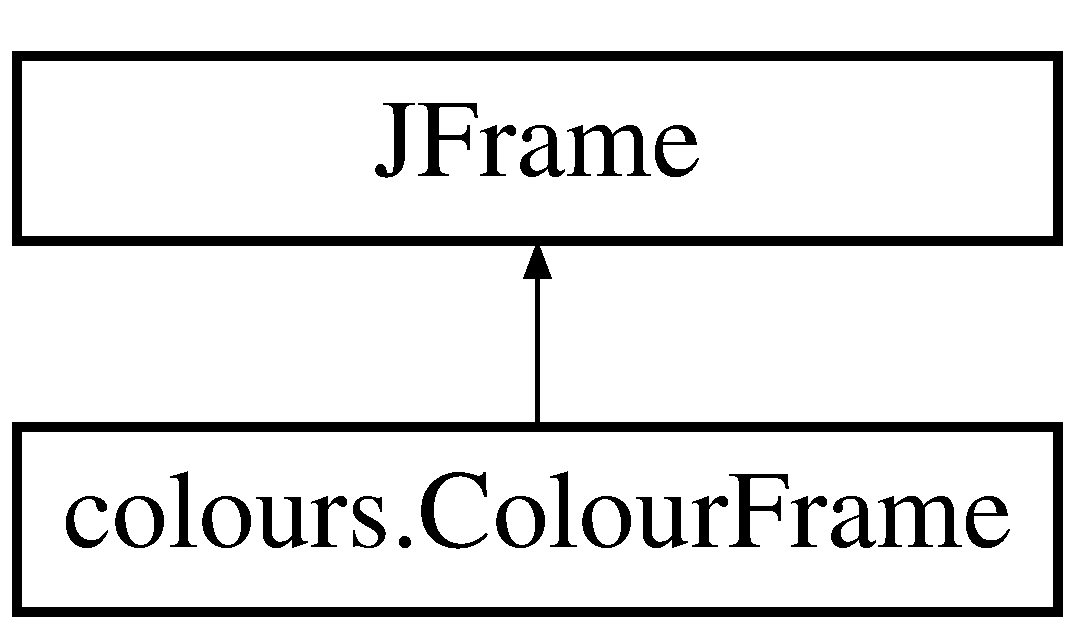
\includegraphics[height=2.000000cm]{classcolours_1_1_colour_frame}
\end{center}
\end{figure}
\subsection*{Public Member Functions}
\begin{DoxyCompactItemize}
\item 
\hyperlink{classcolours_1_1_colour_frame_ab7b3858b7fb97ff26bf7534c1767270c}{Colour\+Frame} ()
\end{DoxyCompactItemize}
\subsection*{Static Public Member Functions}
\begin{DoxyCompactItemize}
\item 
static void \hyperlink{classcolours_1_1_colour_frame_a7f890970aa168fcb9791f1de589a5c2c}{main} (String args\mbox{[}$\,$\mbox{]})
\end{DoxyCompactItemize}
\subsection*{Private Member Functions}
\begin{DoxyCompactItemize}
\item 
void \hyperlink{classcolours_1_1_colour_frame_aa654076ec5e365557e85b7ba8e3dae47}{init\+Components} ()
\item 
void \hyperlink{classcolours_1_1_colour_frame_ad1dd5e41e9cc42f135ff3c1b343ff761}{btn\+Text\+File\+Action\+Performed} (java.\+awt.\+event.\+Action\+Event evt)
\item 
void \hyperlink{classcolours_1_1_colour_frame_ab959355834a40b99a18e05e5121417c5}{btn\+Json\+File\+Action\+Performed} (java.\+awt.\+event.\+Action\+Event evt)
\item 
Boolean \hyperlink{classcolours_1_1_colour_frame_a693e820f5c6ea43ce0a862bd751f42c3}{check\+List\+Not\+Empty} ()
\item 
void \hyperlink{classcolours_1_1_colour_frame_a97c8597f65a97de8993a1ab05d39dd44}{display\+Color} (List$<$ \hyperlink{classcolours_1_1_color_rainbow}{Color\+Rainbow} $>$ rainbow)
\end{DoxyCompactItemize}
\subsection*{Private Attributes}
\begin{DoxyCompactItemize}
\item 
javax.\+swing.\+J\+Button \hyperlink{classcolours_1_1_colour_frame_a1fe23149a50772dff538d0004e7cb1ee}{btn\+Json\+File}
\item 
javax.\+swing.\+J\+Button \hyperlink{classcolours_1_1_colour_frame_aeca940071b6ad635188894ab1be05658}{btn\+Text\+File}
\item 
javax.\+swing.\+J\+Label \hyperlink{classcolours_1_1_colour_frame_a3465e8e9a196ae2a3249b5212e954594}{lbl\+Json\+File}
\item 
javax.\+swing.\+J\+Label \hyperlink{classcolours_1_1_colour_frame_a89795e4433199461d0c29f8f2af8e35f}{lbl\+Text\+File}
\item 
javax.\+swing.\+J\+List$<$ String $>$ \hyperlink{classcolours_1_1_colour_frame_a9c6b0ac09f52427530bd1e0fbc285cc2}{list\+Colour}
\item 
javax.\+swing.\+J\+Scroll\+Pane \hyperlink{classcolours_1_1_colour_frame_a4101dbab121b9af67cb0ff9ef3c64a7a}{scroll\+Pane}
\item 
javax.\+swing.\+J\+Text\+Field \hyperlink{classcolours_1_1_colour_frame_adaffa1254ad772940748d49324e191a0}{txt\+Json\+File}
\item 
javax.\+swing.\+J\+Text\+Field \hyperlink{classcolours_1_1_colour_frame_a8acb908d5dbadca9e110960051340977}{txt\+Text\+File}
\end{DoxyCompactItemize}


\subsection{Detailed Description}
\hyperlink{classcolours_1_1_colour_frame}{Colour\+Frame} --- Main class that use for displaying the G\+UI form. \begin{DoxyAuthor}{Author}
Van Do 
\end{DoxyAuthor}
\begin{DoxyVersion}{Version}
1.\+0 
\end{DoxyVersion}


\subsection{Constructor \& Destructor Documentation}
\mbox{\Hypertarget{classcolours_1_1_colour_frame_ab7b3858b7fb97ff26bf7534c1767270c}\label{classcolours_1_1_colour_frame_ab7b3858b7fb97ff26bf7534c1767270c}} 
\index{colours\+::\+Colour\+Frame@{colours\+::\+Colour\+Frame}!Colour\+Frame@{Colour\+Frame}}
\index{Colour\+Frame@{Colour\+Frame}!colours\+::\+Colour\+Frame@{colours\+::\+Colour\+Frame}}
\subsubsection{\texorpdfstring{Colour\+Frame()}{ColourFrame()}}
{\footnotesize\ttfamily colours.\+Colour\+Frame.\+Colour\+Frame (\begin{DoxyParamCaption}{ }\end{DoxyParamCaption})\hspace{0.3cm}{\ttfamily [inline]}}

The null constructor for the main class. Creates new form. 

\subsection{Member Function Documentation}
\mbox{\Hypertarget{classcolours_1_1_colour_frame_ab959355834a40b99a18e05e5121417c5}\label{classcolours_1_1_colour_frame_ab959355834a40b99a18e05e5121417c5}} 
\index{colours\+::\+Colour\+Frame@{colours\+::\+Colour\+Frame}!btn\+Json\+File\+Action\+Performed@{btn\+Json\+File\+Action\+Performed}}
\index{btn\+Json\+File\+Action\+Performed@{btn\+Json\+File\+Action\+Performed}!colours\+::\+Colour\+Frame@{colours\+::\+Colour\+Frame}}
\subsubsection{\texorpdfstring{btn\+Json\+File\+Action\+Performed()}{btnJsonFileActionPerformed()}}
{\footnotesize\ttfamily void colours.\+Colour\+Frame.\+btn\+Json\+File\+Action\+Performed (\begin{DoxyParamCaption}\item[{java.\+awt.\+event.\+Action\+Event}]{evt }\end{DoxyParamCaption})\hspace{0.3cm}{\ttfamily [inline]}, {\ttfamily [private]}}

This method called a J\+S\+O\+N-\/formatted file and display color details from another frame. 
\begin{DoxyParams}{Parameters}
{\em evt} & -\/ event happened in button. \\
\hline
\end{DoxyParams}
\mbox{\Hypertarget{classcolours_1_1_colour_frame_ad1dd5e41e9cc42f135ff3c1b343ff761}\label{classcolours_1_1_colour_frame_ad1dd5e41e9cc42f135ff3c1b343ff761}} 
\index{colours\+::\+Colour\+Frame@{colours\+::\+Colour\+Frame}!btn\+Text\+File\+Action\+Performed@{btn\+Text\+File\+Action\+Performed}}
\index{btn\+Text\+File\+Action\+Performed@{btn\+Text\+File\+Action\+Performed}!colours\+::\+Colour\+Frame@{colours\+::\+Colour\+Frame}}
\subsubsection{\texorpdfstring{btn\+Text\+File\+Action\+Performed()}{btnTextFileActionPerformed()}}
{\footnotesize\ttfamily void colours.\+Colour\+Frame.\+btn\+Text\+File\+Action\+Performed (\begin{DoxyParamCaption}\item[{java.\+awt.\+event.\+Action\+Event}]{evt }\end{DoxyParamCaption})\hspace{0.3cm}{\ttfamily [inline]}, {\ttfamily [private]}}

Click on this button to display colors details from another frame from a text file. 
\begin{DoxyParams}{Parameters}
{\em evt} & -\/ event happened in button. \\
\hline
\end{DoxyParams}
\mbox{\Hypertarget{classcolours_1_1_colour_frame_a693e820f5c6ea43ce0a862bd751f42c3}\label{classcolours_1_1_colour_frame_a693e820f5c6ea43ce0a862bd751f42c3}} 
\index{colours\+::\+Colour\+Frame@{colours\+::\+Colour\+Frame}!check\+List\+Not\+Empty@{check\+List\+Not\+Empty}}
\index{check\+List\+Not\+Empty@{check\+List\+Not\+Empty}!colours\+::\+Colour\+Frame@{colours\+::\+Colour\+Frame}}
\subsubsection{\texorpdfstring{check\+List\+Not\+Empty()}{checkListNotEmpty()}}
{\footnotesize\ttfamily Boolean colours.\+Colour\+Frame.\+check\+List\+Not\+Empty (\begin{DoxyParamCaption}{ }\end{DoxyParamCaption})\hspace{0.3cm}{\ttfamily [inline]}, {\ttfamily [private]}}

Check to see the list is not empty. \mbox{\Hypertarget{classcolours_1_1_colour_frame_a97c8597f65a97de8993a1ab05d39dd44}\label{classcolours_1_1_colour_frame_a97c8597f65a97de8993a1ab05d39dd44}} 
\index{colours\+::\+Colour\+Frame@{colours\+::\+Colour\+Frame}!display\+Color@{display\+Color}}
\index{display\+Color@{display\+Color}!colours\+::\+Colour\+Frame@{colours\+::\+Colour\+Frame}}
\subsubsection{\texorpdfstring{display\+Color()}{displayColor()}}
{\footnotesize\ttfamily void colours.\+Colour\+Frame.\+display\+Color (\begin{DoxyParamCaption}\item[{List$<$ \hyperlink{classcolours_1_1_color_rainbow}{Color\+Rainbow} $>$}]{rainbow }\end{DoxyParamCaption})\hspace{0.3cm}{\ttfamily [inline]}, {\ttfamily [private]}}

Display front end G\+UI frame to the user to show all colors data from the list. 
\begin{DoxyParams}{Parameters}
{\em rainbow} & -\/ a list of \hyperlink{classcolours_1_1_color_rainbow}{Color\+Rainbow} object from file that deserialize and serialize from J\+S\+ON string. \\
\hline
\end{DoxyParams}

\begin{DoxyExceptions}{Exceptions}
{\em Number\+Format\+Exception} & -\/ catch errors when the conversion between hex code and color has been failed. \\
\hline
\end{DoxyExceptions}
\mbox{\Hypertarget{classcolours_1_1_colour_frame_aa654076ec5e365557e85b7ba8e3dae47}\label{classcolours_1_1_colour_frame_aa654076ec5e365557e85b7ba8e3dae47}} 
\index{colours\+::\+Colour\+Frame@{colours\+::\+Colour\+Frame}!init\+Components@{init\+Components}}
\index{init\+Components@{init\+Components}!colours\+::\+Colour\+Frame@{colours\+::\+Colour\+Frame}}
\subsubsection{\texorpdfstring{init\+Components()}{initComponents()}}
{\footnotesize\ttfamily void colours.\+Colour\+Frame.\+init\+Components (\begin{DoxyParamCaption}{ }\end{DoxyParamCaption})\hspace{0.3cm}{\ttfamily [inline]}, {\ttfamily [private]}}

This method is called from within the constructor to initialize the form. W\+A\+R\+N\+I\+NG\+: Do N\+OT modify this code. The content of this method is always regenerated by the Form Editor. \mbox{\Hypertarget{classcolours_1_1_colour_frame_a7f890970aa168fcb9791f1de589a5c2c}\label{classcolours_1_1_colour_frame_a7f890970aa168fcb9791f1de589a5c2c}} 
\index{colours\+::\+Colour\+Frame@{colours\+::\+Colour\+Frame}!main@{main}}
\index{main@{main}!colours\+::\+Colour\+Frame@{colours\+::\+Colour\+Frame}}
\subsubsection{\texorpdfstring{main()}{main()}}
{\footnotesize\ttfamily static void colours.\+Colour\+Frame.\+main (\begin{DoxyParamCaption}\item[{String}]{args\mbox{[}$\,$\mbox{]} }\end{DoxyParamCaption})\hspace{0.3cm}{\ttfamily [inline]}, {\ttfamily [static]}}


\begin{DoxyParams}{Parameters}
{\em args} & -\/ the command line arguments \\
\hline
\end{DoxyParams}


\subsection{Member Data Documentation}
\mbox{\Hypertarget{classcolours_1_1_colour_frame_a1fe23149a50772dff538d0004e7cb1ee}\label{classcolours_1_1_colour_frame_a1fe23149a50772dff538d0004e7cb1ee}} 
\index{colours\+::\+Colour\+Frame@{colours\+::\+Colour\+Frame}!btn\+Json\+File@{btn\+Json\+File}}
\index{btn\+Json\+File@{btn\+Json\+File}!colours\+::\+Colour\+Frame@{colours\+::\+Colour\+Frame}}
\subsubsection{\texorpdfstring{btn\+Json\+File}{btnJsonFile}}
{\footnotesize\ttfamily javax.\+swing.\+J\+Button colours.\+Colour\+Frame.\+btn\+Json\+File\hspace{0.3cm}{\ttfamily [private]}}

\mbox{\Hypertarget{classcolours_1_1_colour_frame_aeca940071b6ad635188894ab1be05658}\label{classcolours_1_1_colour_frame_aeca940071b6ad635188894ab1be05658}} 
\index{colours\+::\+Colour\+Frame@{colours\+::\+Colour\+Frame}!btn\+Text\+File@{btn\+Text\+File}}
\index{btn\+Text\+File@{btn\+Text\+File}!colours\+::\+Colour\+Frame@{colours\+::\+Colour\+Frame}}
\subsubsection{\texorpdfstring{btn\+Text\+File}{btnTextFile}}
{\footnotesize\ttfamily javax.\+swing.\+J\+Button colours.\+Colour\+Frame.\+btn\+Text\+File\hspace{0.3cm}{\ttfamily [private]}}

\mbox{\Hypertarget{classcolours_1_1_colour_frame_a3465e8e9a196ae2a3249b5212e954594}\label{classcolours_1_1_colour_frame_a3465e8e9a196ae2a3249b5212e954594}} 
\index{colours\+::\+Colour\+Frame@{colours\+::\+Colour\+Frame}!lbl\+Json\+File@{lbl\+Json\+File}}
\index{lbl\+Json\+File@{lbl\+Json\+File}!colours\+::\+Colour\+Frame@{colours\+::\+Colour\+Frame}}
\subsubsection{\texorpdfstring{lbl\+Json\+File}{lblJsonFile}}
{\footnotesize\ttfamily javax.\+swing.\+J\+Label colours.\+Colour\+Frame.\+lbl\+Json\+File\hspace{0.3cm}{\ttfamily [private]}}

\mbox{\Hypertarget{classcolours_1_1_colour_frame_a89795e4433199461d0c29f8f2af8e35f}\label{classcolours_1_1_colour_frame_a89795e4433199461d0c29f8f2af8e35f}} 
\index{colours\+::\+Colour\+Frame@{colours\+::\+Colour\+Frame}!lbl\+Text\+File@{lbl\+Text\+File}}
\index{lbl\+Text\+File@{lbl\+Text\+File}!colours\+::\+Colour\+Frame@{colours\+::\+Colour\+Frame}}
\subsubsection{\texorpdfstring{lbl\+Text\+File}{lblTextFile}}
{\footnotesize\ttfamily javax.\+swing.\+J\+Label colours.\+Colour\+Frame.\+lbl\+Text\+File\hspace{0.3cm}{\ttfamily [private]}}

\mbox{\Hypertarget{classcolours_1_1_colour_frame_a9c6b0ac09f52427530bd1e0fbc285cc2}\label{classcolours_1_1_colour_frame_a9c6b0ac09f52427530bd1e0fbc285cc2}} 
\index{colours\+::\+Colour\+Frame@{colours\+::\+Colour\+Frame}!list\+Colour@{list\+Colour}}
\index{list\+Colour@{list\+Colour}!colours\+::\+Colour\+Frame@{colours\+::\+Colour\+Frame}}
\subsubsection{\texorpdfstring{list\+Colour}{listColour}}
{\footnotesize\ttfamily javax.\+swing.\+J\+List$<$String$>$ colours.\+Colour\+Frame.\+list\+Colour\hspace{0.3cm}{\ttfamily [private]}}

\mbox{\Hypertarget{classcolours_1_1_colour_frame_a4101dbab121b9af67cb0ff9ef3c64a7a}\label{classcolours_1_1_colour_frame_a4101dbab121b9af67cb0ff9ef3c64a7a}} 
\index{colours\+::\+Colour\+Frame@{colours\+::\+Colour\+Frame}!scroll\+Pane@{scroll\+Pane}}
\index{scroll\+Pane@{scroll\+Pane}!colours\+::\+Colour\+Frame@{colours\+::\+Colour\+Frame}}
\subsubsection{\texorpdfstring{scroll\+Pane}{scrollPane}}
{\footnotesize\ttfamily javax.\+swing.\+J\+Scroll\+Pane colours.\+Colour\+Frame.\+scroll\+Pane\hspace{0.3cm}{\ttfamily [private]}}

\mbox{\Hypertarget{classcolours_1_1_colour_frame_adaffa1254ad772940748d49324e191a0}\label{classcolours_1_1_colour_frame_adaffa1254ad772940748d49324e191a0}} 
\index{colours\+::\+Colour\+Frame@{colours\+::\+Colour\+Frame}!txt\+Json\+File@{txt\+Json\+File}}
\index{txt\+Json\+File@{txt\+Json\+File}!colours\+::\+Colour\+Frame@{colours\+::\+Colour\+Frame}}
\subsubsection{\texorpdfstring{txt\+Json\+File}{txtJsonFile}}
{\footnotesize\ttfamily javax.\+swing.\+J\+Text\+Field colours.\+Colour\+Frame.\+txt\+Json\+File\hspace{0.3cm}{\ttfamily [private]}}

\mbox{\Hypertarget{classcolours_1_1_colour_frame_a8acb908d5dbadca9e110960051340977}\label{classcolours_1_1_colour_frame_a8acb908d5dbadca9e110960051340977}} 
\index{colours\+::\+Colour\+Frame@{colours\+::\+Colour\+Frame}!txt\+Text\+File@{txt\+Text\+File}}
\index{txt\+Text\+File@{txt\+Text\+File}!colours\+::\+Colour\+Frame@{colours\+::\+Colour\+Frame}}
\subsubsection{\texorpdfstring{txt\+Text\+File}{txtTextFile}}
{\footnotesize\ttfamily javax.\+swing.\+J\+Text\+Field colours.\+Colour\+Frame.\+txt\+Text\+File\hspace{0.3cm}{\ttfamily [private]}}



The documentation for this class was generated from the following file\+:\begin{DoxyCompactItemize}
\item 
src/colours/\hyperlink{_colour_frame_8java}{Colour\+Frame.\+java}\end{DoxyCompactItemize}

\hypertarget{classcolours_1_1_read_file}{}\section{colours.\+Read\+File Class Reference}
\label{classcolours_1_1_read_file}\index{colours.\+Read\+File@{colours.\+Read\+File}}
\subsection*{Public Member Functions}
\begin{DoxyCompactItemize}
\item 
List$<$ \hyperlink{classcolours_1_1_color_rainbow}{Color\+Rainbow} $>$ \hyperlink{classcolours_1_1_read_file_a6b240cdce8df090dca527f367bacb95b}{get\+From\+Text\+File} (String file\+Name)
\item 
List$<$ \hyperlink{classcolours_1_1_color_rainbow}{Color\+Rainbow} $>$ \hyperlink{classcolours_1_1_read_file_a66c626180f88d15c7833677481eede05}{get\+From\+Json\+File} (String file\+Name)
\end{DoxyCompactItemize}
\subsection*{Private Attributes}
\begin{DoxyCompactItemize}
\item 
Buffered\+Reader \hyperlink{classcolours_1_1_read_file_a3d7ab6f2517fbc88e36249963255930a}{file}
\item 
List$<$ \hyperlink{classcolours_1_1_color_rainbow}{Color\+Rainbow} $>$ \hyperlink{classcolours_1_1_read_file_ada4823ab03166bb5b0c388b40460fa7d}{list}
\end{DoxyCompactItemize}


\subsection{Detailed Description}
\hyperlink{classcolours_1_1_read_file}{Read\+File} --- This class allows to read text file, including text file in J\+S\+ON format. \begin{DoxyAuthor}{Author}
Van Do 
\end{DoxyAuthor}


\subsection{Member Function Documentation}
\mbox{\Hypertarget{classcolours_1_1_read_file_a66c626180f88d15c7833677481eede05}\label{classcolours_1_1_read_file_a66c626180f88d15c7833677481eede05}} 
\index{colours\+::\+Read\+File@{colours\+::\+Read\+File}!get\+From\+Json\+File@{get\+From\+Json\+File}}
\index{get\+From\+Json\+File@{get\+From\+Json\+File}!colours\+::\+Read\+File@{colours\+::\+Read\+File}}
\subsubsection{\texorpdfstring{get\+From\+Json\+File()}{getFromJsonFile()}}
{\footnotesize\ttfamily List$<$\hyperlink{classcolours_1_1_color_rainbow}{Color\+Rainbow}$>$ colours.\+Read\+File.\+get\+From\+Json\+File (\begin{DoxyParamCaption}\item[{String}]{file\+Name }\end{DoxyParamCaption})\hspace{0.3cm}{\ttfamily [inline]}}

Read a J\+S\+O\+N-\/formatted file and deserialize the J\+S\+ON string into list of \hyperlink{classcolours_1_1_color_rainbow}{Color\+Rainbow} objects 
\begin{DoxyParams}{Parameters}
{\em file\+Name} & the name of the file you want to read \\
\hline
\end{DoxyParams}
\begin{DoxyReturn}{Returns}
list of \hyperlink{classcolours_1_1_color_rainbow}{Color\+Rainbow} objects 
\end{DoxyReturn}
\mbox{\Hypertarget{classcolours_1_1_read_file_a6b240cdce8df090dca527f367bacb95b}\label{classcolours_1_1_read_file_a6b240cdce8df090dca527f367bacb95b}} 
\index{colours\+::\+Read\+File@{colours\+::\+Read\+File}!get\+From\+Text\+File@{get\+From\+Text\+File}}
\index{get\+From\+Text\+File@{get\+From\+Text\+File}!colours\+::\+Read\+File@{colours\+::\+Read\+File}}
\subsubsection{\texorpdfstring{get\+From\+Text\+File()}{getFromTextFile()}}
{\footnotesize\ttfamily List$<$\hyperlink{classcolours_1_1_color_rainbow}{Color\+Rainbow}$>$ colours.\+Read\+File.\+get\+From\+Text\+File (\begin{DoxyParamCaption}\item[{String}]{file\+Name }\end{DoxyParamCaption})\hspace{0.3cm}{\ttfamily [inline]}}

This method allows to read from a text file and convert the data into a list. 
\begin{DoxyParams}{Parameters}
{\em file\+Name} & the name of the file you want to read from \\
\hline
\end{DoxyParams}
\begin{DoxyReturn}{Returns}
the list of all color data 
\end{DoxyReturn}


\subsection{Member Data Documentation}
\mbox{\Hypertarget{classcolours_1_1_read_file_a3d7ab6f2517fbc88e36249963255930a}\label{classcolours_1_1_read_file_a3d7ab6f2517fbc88e36249963255930a}} 
\index{colours\+::\+Read\+File@{colours\+::\+Read\+File}!file@{file}}
\index{file@{file}!colours\+::\+Read\+File@{colours\+::\+Read\+File}}
\subsubsection{\texorpdfstring{file}{file}}
{\footnotesize\ttfamily Buffered\+Reader colours.\+Read\+File.\+file\hspace{0.3cm}{\ttfamily [private]}}

Read characters from text file \mbox{\Hypertarget{classcolours_1_1_read_file_ada4823ab03166bb5b0c388b40460fa7d}\label{classcolours_1_1_read_file_ada4823ab03166bb5b0c388b40460fa7d}} 
\index{colours\+::\+Read\+File@{colours\+::\+Read\+File}!list@{list}}
\index{list@{list}!colours\+::\+Read\+File@{colours\+::\+Read\+File}}
\subsubsection{\texorpdfstring{list}{list}}
{\footnotesize\ttfamily List$<$\hyperlink{classcolours_1_1_color_rainbow}{Color\+Rainbow}$>$ colours.\+Read\+File.\+list\hspace{0.3cm}{\ttfamily [private]}}

The list of \hyperlink{classcolours_1_1_color_rainbow}{Color\+Rainbow} objects \begin{DoxySeeAlso}{See also}
\hyperlink{classcolours_1_1_color_rainbow}{Color\+Rainbow} 
\end{DoxySeeAlso}


The documentation for this class was generated from the following file\+:\begin{DoxyCompactItemize}
\item 
src/colours/\hyperlink{_read_file_8java}{Read\+File.\+java}\end{DoxyCompactItemize}

\chapter{File Documentation}
\hypertarget{_color_parser_8java}{}\section{src/colours/\+Color\+Parser.java File Reference}
\label{_color_parser_8java}\index{src/colours/\+Color\+Parser.\+java@{src/colours/\+Color\+Parser.\+java}}
\subsection*{Classes}
\begin{DoxyCompactItemize}
\item 
class \hyperlink{classcolours_1_1_color_parser}{colours.\+Color\+Parser}
\end{DoxyCompactItemize}
\subsection*{Packages}
\begin{DoxyCompactItemize}
\item 
package \hyperlink{namespacecolours}{colours}
\end{DoxyCompactItemize}

\hypertarget{_color_rainbow_8java}{}\section{src/colours/\+Color\+Rainbow.java File Reference}
\label{_color_rainbow_8java}\index{src/colours/\+Color\+Rainbow.\+java@{src/colours/\+Color\+Rainbow.\+java}}
\subsection*{Classes}
\begin{DoxyCompactItemize}
\item 
class \hyperlink{classcolours_1_1_color_rainbow}{colours.\+Color\+Rainbow}
\end{DoxyCompactItemize}
\subsection*{Packages}
\begin{DoxyCompactItemize}
\item 
package \hyperlink{namespacecolours}{colours}
\end{DoxyCompactItemize}

\hypertarget{_colour_frame_8java}{}\section{src/colours/\+Colour\+Frame.java File Reference}
\label{_colour_frame_8java}\index{src/colours/\+Colour\+Frame.\+java@{src/colours/\+Colour\+Frame.\+java}}
\subsection*{Classes}
\begin{DoxyCompactItemize}
\item 
class \hyperlink{classcolours_1_1_colour_frame}{colours.\+Colour\+Frame}
\end{DoxyCompactItemize}
\subsection*{Packages}
\begin{DoxyCompactItemize}
\item 
package \hyperlink{namespacecolours}{colours}
\end{DoxyCompactItemize}

\hypertarget{_read_file_8java}{}\section{src/colours/\+Read\+File.java File Reference}
\label{_read_file_8java}\index{src/colours/\+Read\+File.\+java@{src/colours/\+Read\+File.\+java}}
\subsection*{Classes}
\begin{DoxyCompactItemize}
\item 
class \hyperlink{classcolours_1_1_read_file}{colours.\+Read\+File}
\end{DoxyCompactItemize}
\subsection*{Packages}
\begin{DoxyCompactItemize}
\item 
package \hyperlink{namespacecolours}{colours}
\end{DoxyCompactItemize}

%--- End generated contents ---

% Index
\backmatter
\newpage
\phantomsection
\clearemptydoublepage
\addcontentsline{toc}{chapter}{Index}
\printindex

\end{document}
